\chapter{Clasificación de estrellas RRL utilizando Random Forest}

El objetivo de esta sección es determinar la performance de clasificadores Random Forest aplicados a la tarea de clasificar estrellas variables de tipo RRL. Estos resultados serán utilizados como punto de referencia en secciones posteriores, donde se trabajará con clasificadores basados en Support Vector Machines sobre los mismos datos. La implementacion de Random Forest utilizada es la provista por Scikit-Learn \cite{sklearn_api} \cite{pedregosa2011scikit}.

\section{Optimización de hiperparámetros}

Se realizó un experimento utilizando una metodología muy similar a la descripta en la sección ``Model Selection" de \cite{jbc}. En primer lugar, se optimizaron los hiperparámetros de Random Forest utilizando 10-fold Cross Validation Grid Search sobre el tile b278. Los hiperaparámetros a optimizar fueron:

\begin{itemize}
\item \textbf{$n\_estimators$}: El número de árboles en cada ensamble. Se exploró un amplio rango de valores entre 10 y 750 árboles.
\item \textbf{$max\_features$}: El número de features a considerar cuando se busca el mejor split. Las opciones exploradas fueron la raíz cuadrada del número de features (``sqrt"), y el logaritmo en base dos del número de features (``log2").
\item \textbf{$criterion$}: La función utilizada para medir la calidad de cada split. Las opciones consideradas fueron Gini Impurity (``gini") e Information Gain (``entropy")
\end{itemize}

La medida de performance utilizada fue el área bajo la curva de precision-recall. Los resultados completos pueden observarse en la figura \ref{fig:optimisationrf}. Las siguientes conclusiones se desprenden de este experimento:

\begin{itemize}
\item Utilizar entropy como criterion es consistentemente más beneficioso que utilizar gini.
\item A partir de aproximadamente 200 árboles, la ganancia de agregar más árboles al ensamble es muy pequeña. A partir de aproximadamente 400 árboles, la ganancia de agregar más árboles parece ser nula.
\item Los hiperparámetros óptimos resultaron ser: $criterion$=``entropy", $n\_estimators$=400 y $max\_features$=``sqrt"
\end{itemize}

\begin{figure}[h!]
\begin{center}
  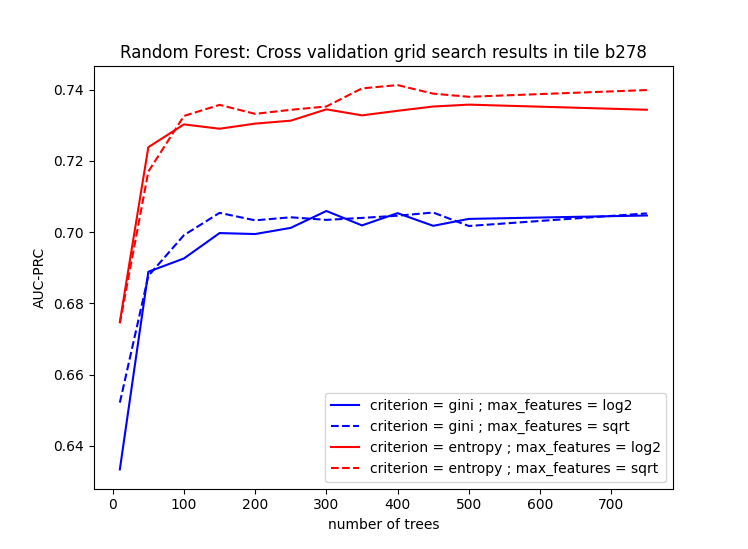
\includegraphics[width=.6\textwidth]{Kap2/Figure_1.png}
  \end{center}
  \caption{Resultados de la optimización de hiperparámetros de Random Forest en el tile b278}
  \label{fig:optimisationrf}
\end{figure}

\section{ Análisis de performance de Random Forest }

Para estimar la performance de Random Forest utilizando los parámetros óptimos que se obtuvieron en la sección anterior, se utilizará un subconjunto fijo de tiles: \{ b234, b261 , b278, b360 \}. Este subconjunto de tiles fue escogido como un compromiso entre la densidad y cobertura de estrellas de tipo RRL\cite{jbc}. Para cada par de tiles $t_1$ y $t_2$, se entrenará un clasificador Random Forest utilizando $t_1$ como dataset de training y $t_2$ como dataset de test, obteniendo curvas de precision-recall. \\

Las curvas resultantes pueden observarse en la figura \ref{fig:testresults}, en color azul. Los valores obtenidos son consistentes con aquellos reportados en trabajos previos \cite{jbc}. Pueden observarse diversos comportamientos, dependiendo de los datos de training y testing seleccionados. En la mayoría de los casos, parece ser posible fijar un recall de 0.5 y obtener una precisión igual o mayor a 0.5. Si se desea una mayor precisión, por ejemplo 0.9; parece ser posible fijar un recall de 0.2 para obtenerla. Esto significa que, utilizando random forests, sería posible detectar automáticamente y con alta precisión al menos el 20\% de las RLL mapeadas por el VVV.



\begin{comment}


\begin{figure}[h]
\begin{center}

\begin{tabular}{ccc}

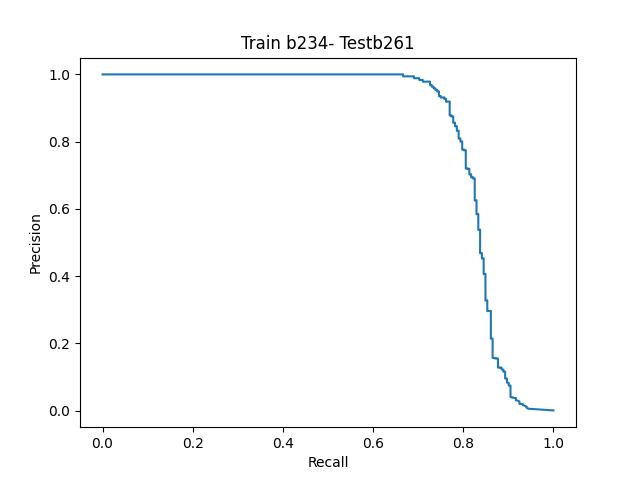
\includegraphics[width=0.32\textwidth]{"Kap2/rf_test_results_train=b234Test=b261.png"} &
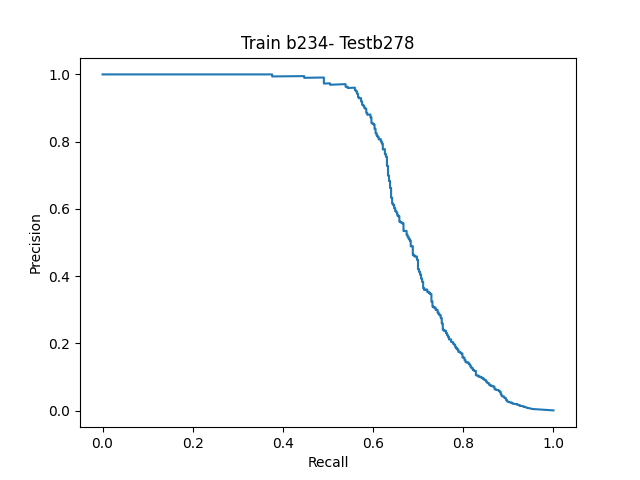
\includegraphics[width=0.32\textwidth]{"Kap2/rf_test_results_train=b234Test=b278.png"} &
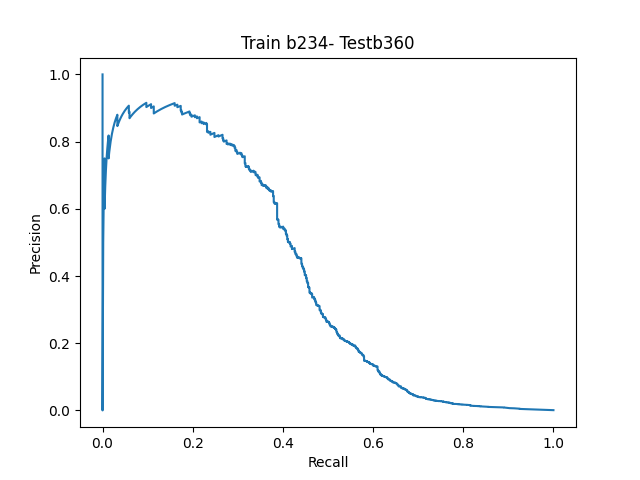
\includegraphics[width=0.32\textwidth]{"Kap2/rf_test_results_train=b234Test=b360.png"} \\

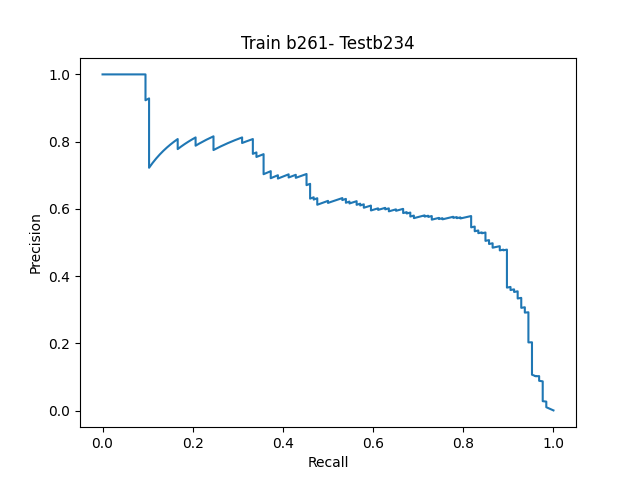
\includegraphics[width=0.32\textwidth]{"Kap2/rf_test_results_train=b261Test=b234.png"} &
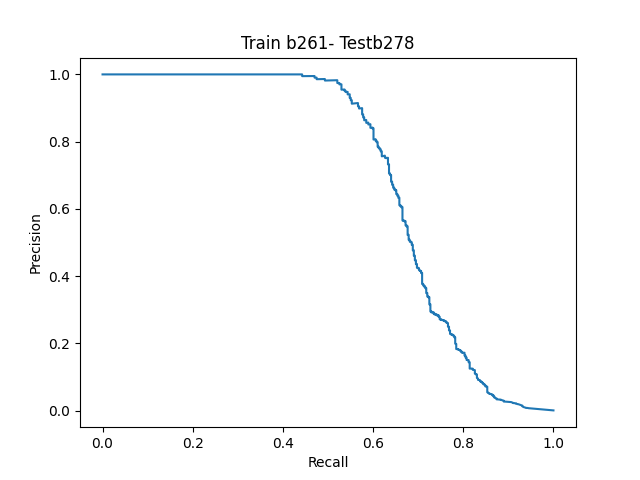
\includegraphics[width=0.32\textwidth]{"Kap2/rf_test_results_train=b261Test=b278.png"} &
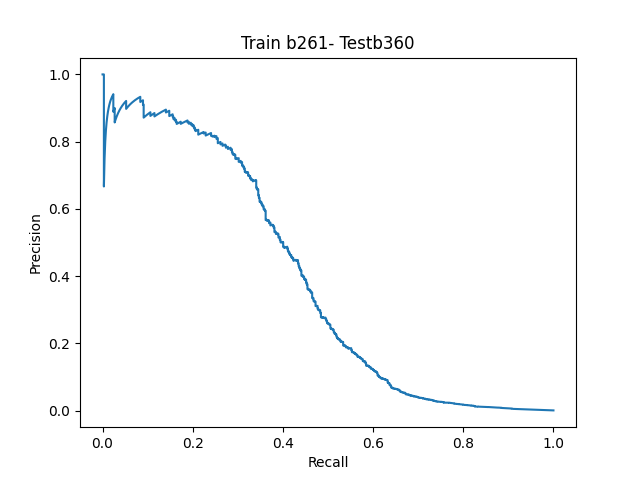
\includegraphics[width=0.32\textwidth]{"Kap2/rf_test_results_train=b261Test=b360.png"} \\

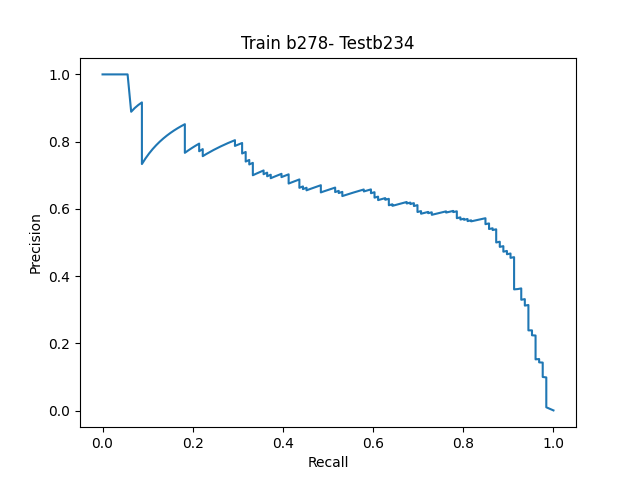
\includegraphics[width=0.32\textwidth]{"Kap2/rf_test_results_train=b278Test=b234.png"} &
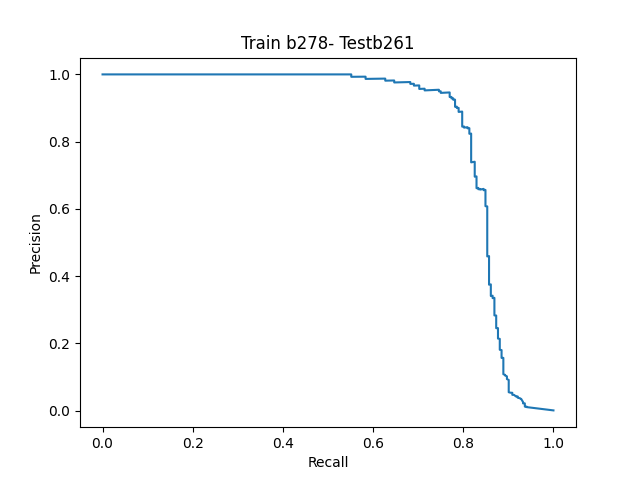
\includegraphics[width=0.32\textwidth]{"Kap2/rf_test_results_train=b278Test=b261.png"} &
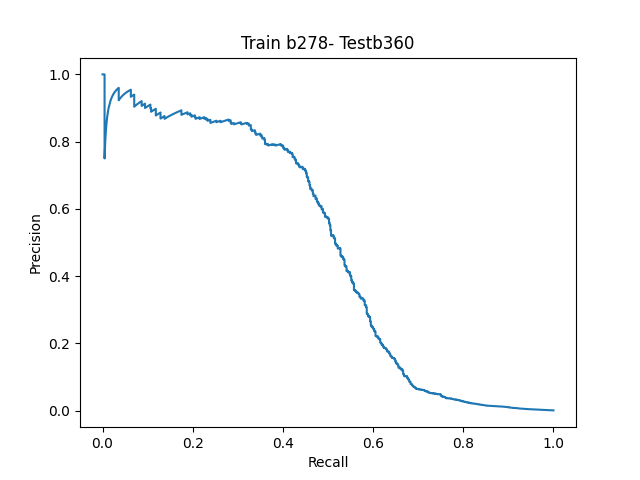
\includegraphics[width=0.32\textwidth]{"Kap2/rf_test_results_train=b278Test=b360.png"} \\

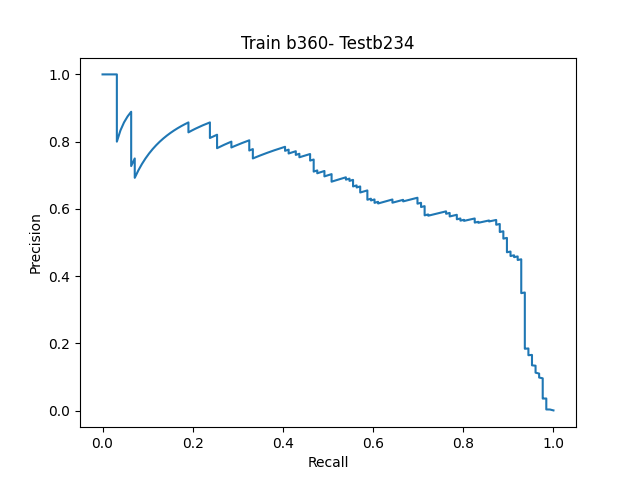
\includegraphics[width=0.32\textwidth]{"Kap2/rf_test_results_train=b360Test=b234.png"} &
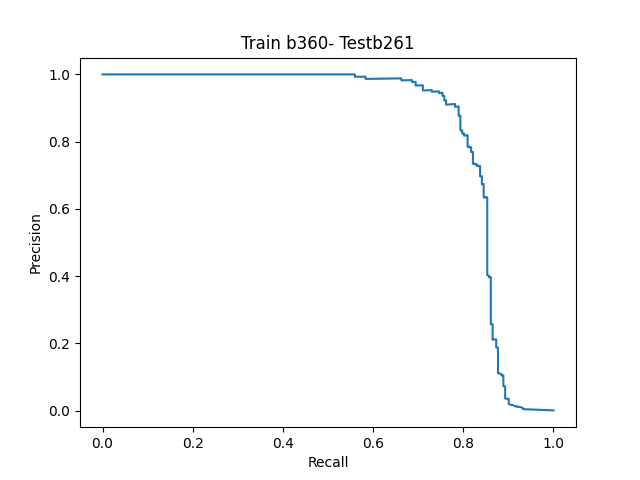
\includegraphics[width=0.32\textwidth]{"Kap2/rf_test_results_train=b360Test=b261.png"} &
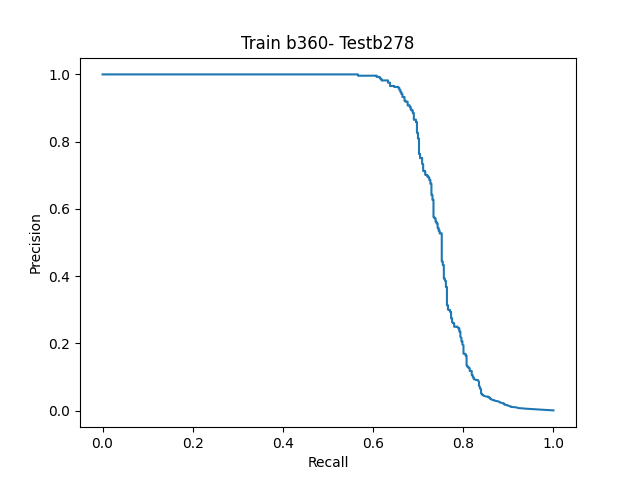
\includegraphics[width=0.32\textwidth]{"Kap2/rf_test_results_train=b360Test=b278.png"}

\end{tabular}

\end{center}
\caption[short]{Curvas de precision-recall obtenidas utilizando Random Forest}
\label{fig:testresultsrf}
\end{figure}


\end{comment}

